
\chapter[Máy quang phổ]{Máy quang phổ}

\section{Lý thuyết}
Máy quang phổ là dụng cụ để phân tích một chùm ánh sáng phức tạp thành những thành phần đơn sắc.
\subsection{Cấu tạo}
Máy quang phổ lăng kính gồm 3 bộ phận chính: ống chuẩn trực, hệ tán sắc và buồng ảnh.
\begin{description}
	\item[Ống chuẩn trực] gồm hệ thấu kính đặt đồng trục, có tác dụng làm chùm sáng từ vật cần đo qua ống cho chùm tia ló song song.
	\item[Hệ tán sắc] gồm một lăng kính (hoặc hệ lăng kính), có tác dụng phân tách chùm sáng song song khi qua ống chuẩn trực thành nhiều chùm tia đơn sắc, song song.
	\item[Buồng tối (buồng ảnh)] là một hộp kín có chứa kính ảnh đặt tại tiêu diện ảnh của thấu kính hội tụ, có tác dụng quan sát quang phổ.
\end{description} 	
\begin{center}
	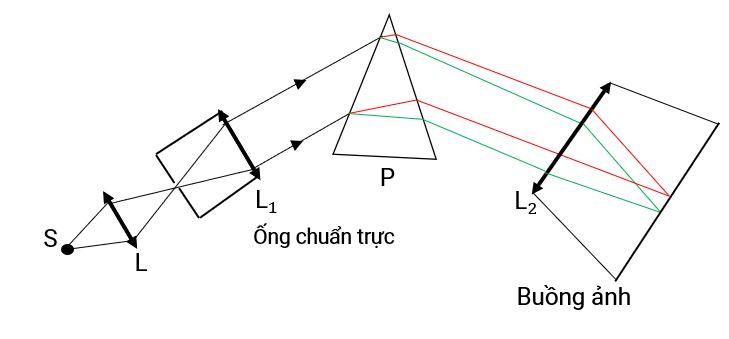
\includegraphics[scale=1]{../figs/VN12-PH-36-L-021-1-1.JPG}
\end{center}
\subsection{Nguyên tắc hoạt động}
Nguyên tắc hoạt động của máy quang phổ lăng kính dựa trên hiện tượng tán sắc ánh sáng.
\begin{itemize}
	
	\item Sau khi ló ra khỏi ống chuẩn trực, chùm ánh sáng sẽ trở thành một chùm song song. 
	
	\item Chùm này qua lăng kính sẽ bị phân tách thành nhiều chùm đơn sắc song song, lệch theo các phương khác nhau. 
	
	\item Mỗi chùm sáng đơn sắc được thấu kính hội tụ thành một vạch trên tiêu diện, đó là một vạch màu. 
	
	\item Các vạch màu này được chụp trên kính ảnh hoặc hiện lên tấm kính mờ. Mỗi vạch màu ứng với một bước sóng xác định, gọi là vạch quang phổ. 
	\item Tập hợp các vạch quang phổ chụp được làm thành quang phổ của nguồn.
	
\end{itemize}
\section{Bài tập tự luyện}
\begin{enumerate}[label=\bfseries Câu \arabic*:]
	
	%========================================
	\item \mkstar{1} [2]
	\cauhoi
	{Khe sáng của ống chuẩn trực của máy quang phổ được đặt tại
		\begin{mcq}(1)
			\item một điểm trên trục chính. 
			\item quang tâm của thấu kính hội tụ.
			\item tiêu điểm ảnh của thấu kính hội tụ. 
			\item tiêu điểm vật chính của thấu kính hội tụ. 
		\end{mcq}
	}
	
	\loigiai
	{		\textbf{Đáp án: D.}
		
		Khe sáng của ống chuẩn trực của máy quang phổ được đặt tại tiêu điểm vật chính của thấu kính hội tụ.
	}
	
	%========================================
	\item \mkstar{1} [3]
	\cauhoi
	{Nguyên tắc hoạt động của máy quang phổ lăng kính dựa vào hiện tượng
		\begin{mcq}(2)
			\item tán sắc ánh sáng.
			\item phản xạ toàn phần. 
			\item khúc xạ ánh sáng.
			\item giao thoa ánh sáng. 
		\end{mcq}
	}
	
	\loigiai
	{		\textbf{Đáp án: A.}
		
		Nguyên tắc hoạt động của máy quang phổ lăng kính dựa vào hiện tượng tán sắc ánh sáng.
	}
	
	%========================================
	\item \mkstar{1} [4]
	\cauhoi
	{Ống chuẩn trực trong máy quang phổ có tác dụng 
		\begin{mcq}(1)
			\item tạo ra chùm tia hội tụ. 
			\item tạo ra chùm sáng song song. 
			\item tạo ra chùm tia phân kì. 
			\item tách chùm sáng phức tạp thành nhiều thành phần. 
		\end{mcq}
	}
	
	\loigiai
	{		\textbf{Đáp án: B.}
		
		Ống chuẩn trực trong máy quang phổ có tác dụng tạo ra chùm sáng song song. 
	}
	
	%========================================
	\item \mkstar{1} [13]
	\cauhoi
	{Máy quang phổ lăng kính gồm các bộ phận chính
		\begin{mcq}(1)
			\item ống chuẩn trực, thấu kính, buồng tối. 
			\item ống chuẩn trực, hệ tán sắc, lăng kính. 
			\item thấu kính phân kì, hệ tán sắc, buồng tối. 
			\item ống chuẩn trực, hệ tán sắc, buồng tối. 
		\end{mcq}
	}
	
	\loigiai
	{		\textbf{Đáp án: D.}
		
		Máy quang phổ lăng kính gồm các bộ phận chính ống chuẩn trực, hệ tán sắc, buồng tối.
	}
	
	%========================================
	\item \mkstar{1} [9]
	\cauhoi
	{Bộ phận có tác dụng phân tích chùm sáng phức tạp thành phần đơn sắc trong máy quang phổ lăng kính là 
		\begin{mcq}(4)
			\item buồng tối. 
			\item tấm kính ảnh. 
			\item lăng kính. 
			\item ống chuẩn trực. 
		\end{mcq}
	}
	
	\loigiai
	{		\textbf{Đáp án: C.}
		
		Bộ phận có tác dụng phân tích chùm sáng phức tạp thành phần đơn sắc trong máy quang phổ lăng kính là lăng kính. 
	}
	
\end{enumerate}

